\documentclass[12pt]{extarticle}
\usepackage{manualdoprofessor}
\usepackage{fichatecnica}
\usepackage{lipsum,media9,graficos}
\usepackage[justification=raggedright]{caption}
\usepackage[one]{bncc}
\usepackage[hedra]{../edlab}
\usepackage{marginnote}
\usepackage{makeidx,hedraindex}
\usepackage{longtable}
\makeindex	 


\newcommand{\AutorLivro}{}
\newcommand{\TituloLivro}{BNCCs}
\newcommand{\Tema}{}
\newcommand{\Genero}{}
\newcommand{\imagemCapa}{./images/PNLD0001-01.png}
\newcommand{\issnppub}{---}
\newcommand{\issnepub}{---}
% \newcommand{\fichacatalografica}{PNLD0001-00.png}
\newcommand{\colaborador}{}



\begin{document}



\title{\TituloLivro}
\author{\AutorLivro}
\def\authornotes{\colaborador}

\date{}
\maketitle
\tableofcontents


\newcommand{\bnccativividadespreleitura}{
	\BNCC{EM13LGG704}
	\BNCC{EM13LP12}}

\newcommand{\bnccativividadesleitura}{
	\BNCC{EM13LGG103}
	\BNCC{EM13LP02}}

\newcommand{\bnccativividadesposleitura}{
	\BNCC{EM13LGG102}
	\BNCC{EM13LGG303}}

\newcommand{\bnccreferenciasgerais}{
	\BNCC{EM13LGG302}
	\BNCC{EM13LP46}
	\BNCC{EM13LP49}}

\section{Conjunto: Básicos citados nos filmes}

\subsection{Pre-leitura}
\bnccativividadespreleitura
\subsection{Leitura}
\bnccativividadesleitura
\subsection{Pos-leitura}
\bnccativividadesposleitura
\subsection{Generico}
\bnccreferenciasgerais

\section{Subconjuntos}
\subsection{POEMA}
\subsubsection{Pre-leitura}
\BNCC{EM13LP30} \BNCC{EM13CHS502} \BNCC{EM13CHS103} 
\subsubsection{Leitura}
\BNCC{EM13LGG401} \BNCC{EM13LGG101} \BNCC{EM13LP15} \BNCC{EM13LP09}
\subsubsection{Pos-leitura}
\BNCC{EM13LP50} \BNCC{EM13LGG601} \BNCC{EM13LP53} \BNCC{EM13LGG604}
\subsubsection{Generico}
\BNCC{EM13LGG203} \BNCC{EM13LGG204}

\subsection{CONTO}
\subsubsection{Pre-leitura}
\BNCC{EM13LP32} \BNCC{EM13LGG202} \BNCC{EM13LP30}
\subsubsection{Leitura}
\BNCC{EM13LP15} \BNCC{EM13LP09} \BNCC{EM13LGG401}
\subsubsection{Pos-leitura}
\BNCC{EM13LGG601} \BNCC{EM13LP51} \BNCC{EM13LGG104} \BNCC{EM13LP53}
\subsubsection{Generico}
\BNCC{EM13LGG204} \BNCC{EM13LGG20}

\subsection{ROMANCE}
\subsubsection{Pre-leitura}
\BNCC{EM13CHS502} \BNCC{EM13LP32} \BNCC{EM13CHS103}	 
\subsubsection{Leitura}
\BNCC{EM13LGG401} \BNCC{EM13LP01} \BNCC{EM13LP07}		 
\subsubsection{Pos-leitura}
\BNCC{EM13LGG604} \BNCC{EM13CHS102} 
\subsubsection{Generico}
\BNCC{EM13CHS502} \BNCC{EM13LGG203} \BNCC{EM13LGG602} 						%

\subsection{DIARIO}
\subsubsection{Pre-leitura}
\BNCC{EM13LP30} \BNCC{EM13CHS102} \BNCC{EM13CHS502}			 
\subsubsection{Leitura}
\BNCC{EM13LP01} \BNCC{EM13CHS503}  \BNCC{EM13LGG401}
\subsubsection{Pos-leitura}
\BNCC{EM13LGG601} \BNCC{EM13CHS103} 
\subsubsection{Generico}
\BNCC{EM13LGG101} \BNCC{EM13LGG203} 

\section{Conceitos}

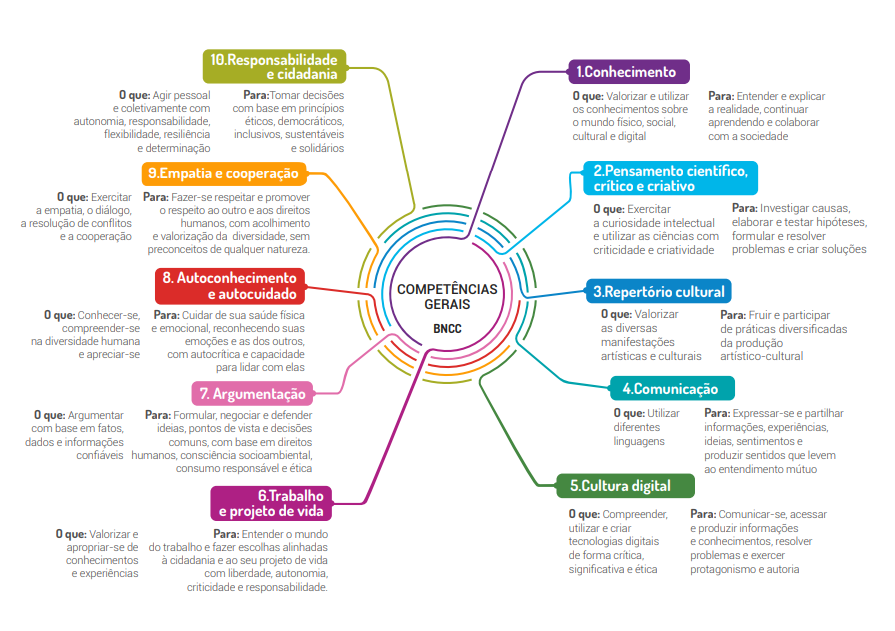
\includegraphics[width=1.2\textwidth]{./images/BNCC-01}
\Image{}{BNCC-02}
\Image{}{BNCC-03}
%\Image{}{BNCC-04}
\Image{}{BNCC-05}


\pagebreak
\section{Todos}
\setcounter{themycounter}{0}
\BNCC{EM13CNT310}
\BNCC{EM13LGG101}
\BNCC{EM13LGG102}
\BNCC{EM13LGG103}
\BNCC{EM13LGG104}
\BNCC{EM13LGG201}
\BNCC{EM13LGG202}
\BNCC{EM13LGG203}
\BNCC{EM13LGG204}
\BNCC{EM13LGG301}
\BNCC{EM13LGG302}
\BNCC{EM13LGG303}
\BNCC{EM13LGG304}
\BNCC{EM13LGG305}
\BNCC{EM13LGG401}
\BNCC{EM13LGG402}
\BNCC{EM13LGG403}
\BNCC{EM13LGG501}
\BNCC{EM13LGG502}
\BNCC{EM13LGG503}
\BNCC{EM13LGG601}
\BNCC{EM13LGG602}
\BNCC{EM13LGG603}
\BNCC{EM13LGG604}
\BNCC{EM13LGG701}
\BNCC{EM13LGG702}
\BNCC{EM13LGG703}
\BNCC{EM13LGG704}
\BNCC{EM13MAT101}
\BNCC{EM13MAT102}
\BNCC{EM13MAT103}
\BNCC{EM13MAT104}
\BNCC{EM13MAT105}
\BNCC{EM13MAT106}
\BNCC{EM13MAT201}
\BNCC{EM13MAT202}
\BNCC{EM13MAT203}
\BNCC{EM13MAT301}
\BNCC{EM13MAT302}
\BNCC{EM13MAT303}
\BNCC{EM13MAT304}
\BNCC{EM13MAT305}
\BNCC{EM13MAT306}
\BNCC{EM13MAT307}
\BNCC{EM13MAT308}
\BNCC{EM13MAT309}
\BNCC{EM13MAT310}
\BNCC{EM13MAT311}
\BNCC{EM13MAT312}
\BNCC{EM13MAT313}
\BNCC{EM13MAT314}
\BNCC{EM13MAT315}
\BNCC{EM13MAT316}
\BNCC{EM13MAT401}
\BNCC{EM13MAT402}
\BNCC{EM13MAT403}
\BNCC{EM13MAT404}
\BNCC{EM13MAT405}
\BNCC{EM13MAT406}
\BNCC{EM13MAT407}
\BNCC{EM13MAT501}
\BNCC{EM13MAT502}
\BNCC{EM13MAT503}
\BNCC{EM13MAT504}
\BNCC{EM13MAT505}
\BNCC{EM13MAT506}
\BNCC{EM13MAT507}
\BNCC{EM13MAT508}
\BNCC{EM13MAT509}
\BNCC{EM13MAT510}
\BNCC{EM13MAT511}
\BNCC{EM13CHS606}
\BNCC{EM13CNT101}
\BNCC{EM13CNT102}
\BNCC{EM13CNT103}
\BNCC{EM13CNT104}
\BNCC{EM13CNT105}
\BNCC{EM13CNT106}
\BNCC{EM13CNT107}
\BNCC{EM13CNT201}
\BNCC{EM13CNT202}
\BNCC{EM13CNT203}
\BNCC{EM13CNT204}
\BNCC{EM13CNT205}
\BNCC{EM13CNT206}
\BNCC{EM13CNT207}
\BNCC{EM13CNT208}
\BNCC{EM13CNT209}
\BNCC{EM13CNT301}
\BNCC{EM13CNT302}
\BNCC{EM13CNT303}
\BNCC{EM13CNT304}
\BNCC{EM13CNT305}
\BNCC{EM13CNT306}
\BNCC{EM13CNT307}
\BNCC{EM13CNT308}
\BNCC{EM13CNT309}
\BNCC{EM13CHS101}
\BNCC{EM13CHS102}
\BNCC{EM13CHS103}
\BNCC{EM13CHS104}
\BNCC{EM13CHS105}
\BNCC{EM13CHS106}
\BNCC{EM13CHS201}
\BNCC{EM13CHS202}
\BNCC{EM13CHS203}
\BNCC{EM13CHS204}
\BNCC{EM13CHS205}
\BNCC{EM13CHS206}
\BNCC{EM13CHS301}
\BNCC{EM13CHS302}
\BNCC{EM13CHS303}
\BNCC{EM13CHS304}
\BNCC{EM13CHS305}
\BNCC{EM13CHS306}
\BNCC{EM13CHS401}
\BNCC{EM13CHS402}
\BNCC{EM13CHS403}
\BNCC{EM13CHS404}
\BNCC{EM13CHS501}
\BNCC{EM13CHS502}
\BNCC{EM13CHS503}
\BNCC{EM13CHS504}
\BNCC{EM13CHS601}
\BNCC{EM13CHS602}
\BNCC{EM13CHS603}
\BNCC{EM13CHS604}
\BNCC{EM13CHS605}
\BNCC{EM13LGG105}
\BNCC{EM13LP01}
\BNCC{EM13LP02}
\BNCC{EM13LP03}
\BNCC{EM13LP04}
\BNCC{EM13LP05}
\BNCC{EM13LP06}
\BNCC{EM13LP07}
\BNCC{EM13LP08}
\BNCC{EM13LP09}
\BNCC{EM13LP10}
\BNCC{EM13LP11}
\BNCC{EM13LP12}
\BNCC{EM13LP13}
\BNCC{EM13LP14}
\BNCC{EM13LP15}
\BNCC{EM13LP16}
\BNCC{EM13LP17}
\BNCC{EM13LP18}
\BNCC{EM13LP19}
\BNCC{EM13LP20}
\BNCC{EM13LP21}
\BNCC{EM13LP22}
\BNCC{EM13LP23}
\BNCC{EM13LP24}
\BNCC{EM13LP25}
\BNCC{EM13LP26}
\BNCC{EM13LP27}
\BNCC{EM13LP28}
\BNCC{EM13LP29}
\BNCC{EM13LP30}
\BNCC{EM13LP31}
\BNCC{EM13LP32}
\BNCC{EM13LP33}
\BNCC{EM13LP34}
\BNCC{EM13LP35}
\BNCC{EM13LP36}
\BNCC{EM13LP37}
\BNCC{EM13LP38}
\BNCC{EM13LP39}
\BNCC{EM13LP40}
\BNCC{EM13LP41}
\BNCC{EM13LP42}
\BNCC{EM13LP43}
\BNCC{EM13LP44}
\BNCC{EM13LP45}
\BNCC{EM13LP46}
\BNCC{EM13LP47}
\BNCC{EM13LP48}
\BNCC{EM13LP49}
\BNCC{EM13LP50}
\BNCC{EM13LP51}
\BNCC{EM13LP52}
\BNCC{EM13LP53}
\BNCC{EM13LP54}


\begin{longtable}{ll}

\rowcolor[HTML]{FFF} 


% Please add the following required packages to your document preamble:
% \usepackage[table,xcdraw]{xcolor}
% If you use beamer only pass "xcolor=table" option, i.e. \documentclass[xcolor=table]{beamer}

EM13CNT310 & serviços básicos; *necessidades locais* e/ou regionais                                                                                                                                                                                                                                                                                                                                                                                                                                                                                                                                                                                                                                                                                                                                                                \\
\rowcolor[HTML]{E0F7FA} 
EM13LGG101 & processos de produção e *circulação de discursos*                                                                                                                                                                                                                                                                                                                                                                                                                                                                                                                                                                                                                                                                                                                                                                     \\
\rowcolor[HTML]{FFF} 
EM13LGG102 & preconceitos e *ideologias* nas diferentes mídias                                                                                                                                                                                                                                                                                                                                                                                                                                                                                                                                                                                                                                                                                                                                                                     \\
\rowcolor[HTML]{E0F7FA} 
EM13LGG103 & *produzir discursos* em textos de diversas semioses                                                                                                                                                                                                                                                                                                                                                                                                                                                                                                                                                                                                                                                                                                                                                                   \\
\rowcolor[HTML]{FFF} 
EM13LGG104 & utilizar diferentes *linguagens* e produção de textos                                                                                                                                                                                                                                                                                                                                                                                                                                                                                                                                                                                                                                                                                                                                                                 \\
\rowcolor[HTML]{E0F7FA} 
EM13LGG201 & diversas linguagens (artísticas, corporais e verbais) em diferentes *contextos*                                                                                                                                                                                                                                                                                                                                                                                                                                                                                                                                                                                                                                                                                                                                       \\
\rowcolor[HTML]{FFF} 
EM13LGG202 & relações de poder e perspectivas de mundo nos discursos, o modo como circulam, *ideologias*.                                                                                                                                                                                                                                                                                                                                                                                                                                                                                                                                                                                                                                                                                                                          \\
\rowcolor[HTML]{E0F7FA} 
EM13LGG203 & analisar disputa por *legitimidade* \textless{}lugardefala\textgreater{}                                                                                                                                                                                                                                                                                                                                                                                                                                                                                                                                                                                                                                                                                                                                              \\
\rowcolor[HTML]{FFF} 
EM13LGG204 & Dialogar e produzir *entendimento mútuo*, \textless{}democracia\textgreater{}                                                                                                                                                                                                                                                                                                                                                                                                                                                                                                                                                                                                                                                                                                                                         \\
\rowcolor[HTML]{E0F7FA} 
EM13LGG301 & produção *individual e colaborativa*                                                                                                                                                                                                                                                                                                                                                                                                                                                                                                                                                                                                                                                                                                                                                                                  \\
\rowcolor[HTML]{FFF} 
EM13LGG302 & *Posicionar-se* criticamente diante de diversas visões de mundo                                                                                                                                                                                                                                                                                                                                                                                                                                                                                                                                                                                                                                                                                                                                                       \\
\rowcolor[HTML]{E0F7FA} 
EM13LGG303 & Debater *questões polêmicas*                                                                                                                                                                                                                                                                                                                                                                                                                                                                                                                                                                                                                                                                                                                                                                                          \\
\rowcolor[HTML]{FFF} 
EM13LGG304 & Formular propostas, intervir e tomar decisões, *Direitos Humanos*, a consciência socioambiental                                                                                                                                                                                                                                                                                                                                                                                                                                                                                                                                                                                                                                                                                                                       \\
\rowcolor[HTML]{E0F7FA} 
EM13LGG305 & *atuação social*, política, artística e cultural                                                                                                                                                                                                                                                                                                                                                                                                                                                                                                                                                                                                                                                                                                                                                                      \\
\rowcolor[HTML]{FFF} 
EM13LGG401 & caracterizar as *línguas* como fenômeno (geo)político, histórico, social                                                                                                                                                                                                                                                                                                                                                                                                                                                                                                                                                                                                                                                                                                                                              \\
\rowcolor[HTML]{E0F7FA} 
EM13LGG402 & *preconceito linguístico*                                                                                                                                                                                                                                                                                                                                                                                                                                                                                                                                                                                                                                                                                                                                                                                             \\
\rowcolor[HTML]{FFF} 
EM13LGG403 & *inglês* como língua de comunicação global                                                                                                                                                                                                                                                                                                                                                                                                                                                                                                                                                                                                                                                                                                                                                                            \\
\rowcolor[HTML]{E0F7FA} 
EM13LGG501 & *práticas corporais*                                                                                                                                                                                                                                                                                                                                                                                                                                                                                                                                                                                                                                                                                                                                                                                                  \\
\rowcolor[HTML]{FFF} 
EM13LGG502 & Analisar criticamente *contra preconceitos*, posicionamento contrário                                                                                                                                                                                                                                                                                                                                                                                                                                                                                                                                                                                                                                                                                                                                                 \\
\rowcolor[HTML]{E0F7FA} 
EM13LGG503 & *cuidado com o corpo* e com a saúde, socialização e entretenimento.                                                                                                                                                                                                                                                                                                                                                                                                                                                                                                                                                                                                                                                                                                                                                   \\
\rowcolor[HTML]{FFF} 
EM13LGG601 & Apropriar-se do *patrimônio artístico*                                                                                                                                                                                                                                                                                                                                                                                                                                                                                                                                                                                                                                                                                                                                                                                \\
\rowcolor[HTML]{E0F7FA} 
EM13LGG602 & Fruir e *apreciar esteticamente*                                                                                                                                                                                                                                                                                                                                                                                                                                                                                                                                                                                                                                                                                                                                                                                      \\
\rowcolor[HTML]{FFF} 
EM13LGG603 & processos de *criação autorais* individuais e coletivos nas diferentes linguagens                                                                                                                                                                                                                                                                                                                                                                                                                                                                                                                                                                                                                                                                                                                                     \\
\rowcolor[HTML]{E0F7FA} 
EM13LGG604 & *práticas artísticas + cultura + histórica*                                                                                                                                                                                                                                                                                                                                                                                                                                                                                                                                                                                                                                                                                                                                                                           \\
\rowcolor[HTML]{FFF} 
EM13LGG701 & Explorar *tecnologias digitais*                                                                                                                                                                                                                                                                                                                                                                                                                                                                                                                                                                                                                                                                                                                                                                                       \\
\rowcolor[HTML]{E0F7FA} 
EM13LGG702 & uso *crítico das mídias digitais*                                                                                                                                                                                                                                                                                                                                                                                                                                                                                                                                                                                                                                                                                                                                                                                     \\
\rowcolor[HTML]{FFF} 
EM13LGG703 & Utilizar *ferramentas digitais* em processos de produção                                                                                                                                                                                                                                                                                                                                                                                                                                                                                                                                                                                                                                                                                                                                                              \\
\rowcolor[HTML]{E0F7FA} 
EM13LGG704 & Apropriar-se de *processos de pesquisa*, ferramentas para distribuição do conhecimento                                                                                                                                                                                                                                                                                                                                                                                                                                                                                                                                                                                                                                                                                                                                \\
\rowcolor[HTML]{FFF} 
EM13MAT101 & Interpretar criticamente situações econômicas, sociais, Ciências da Natureza, *análise dos gráficos*                                                                                                                                                                                                                                                                                                                                                                                                                                                                                                                                                                                                                                                                                                                  \\
\rowcolor[HTML]{E0F7FA} 
EM13MAT102 & Analisar tabelas, gráficos e amostras de pesquisas *estatísticas*                                                                                                                                                                                                                                                                                                                                                                                                                                                                                                                                                                                                                                                                                                                                                     \\
\rowcolor[HTML]{FFF} 
EM13MAT103 & Interpretar e compreender textos científicos                                                                                                                                                                                                                                                                                                                                                                                                                                                                                                                                                                                                                                                                                                                                                                          \\
\rowcolor[HTML]{E0F7FA} 
EM13MAT104 & Interpretar taxas e índices de natureza socioeconômica (índice de desenvolvimento humano, taxas de inflação, entre outros), investigando os processos de cálculo desses números, para analisar criticamente a realidade e produzir argumentos.                                                                                                                                                                                                                                                                                                                                                                                                                                                                                                                                                                        \\
\rowcolor[HTML]{FFF} 
EM13MAT105 & Utilizar as noções de transformações isométricas (translação, reflexão, rotação e composições destas) e transformações homotéticas para construir figuras e analisar elementos da natureza e diferentes produções humanas (fractais, construções civis, obras de arte, entre outras).                                                                                                                                                                                                                                                                                                                                                                                                                                                                                                                                 \\
\rowcolor[HTML]{E0F7FA} 
EM13MAT106 & Identificar situações da vida cotidiana nas quais seja necessário fazer escolhas levando-se em conta os riscos probabilísticos (usar este ou aquele método contraceptivo, optar por um tratamento médico em detrimento de outro etc.).                                                                                                                                                                                                                                                                                                                                                                                                                                                                                                                                                                                \\
\rowcolor[HTML]{FFF} 
EM13MAT201 & Propor ou participar de ações adequadas às demandas da região, preferencialmente para sua comunidade, envolvendo medições e cálculos de perímetro, de área, de volume, de capacidade ou de massa.                                                                                                                                                                                                                                                                                                                                                                                                                                                                                                                                                                                                                     \\
\rowcolor[HTML]{E0F7FA} 
EM13MAT202 & Planejar e executar pesquisa amostral sobre questões relevantes, usando dados coletados diretamente ou em diferentes fontes, e comunicar os resultados por meio de relatório contendo gráficos e interpretação das medidas de tendência central e das medidas de dispersão (amplitude e desvio padrão), utilizando ou não recursos tecnológicos.                                                                                                                                                                                                                                                                                                                                                                                                                                                                      \\
\rowcolor[HTML]{FFF} 
EM13MAT203 & Aplicar conceitos matemáticos no planejamento, na execução e na análise de ações envolvendo a utilização de aplicativos e a criação de planilhas (para o controle de orçamento familiar, simuladores de cálculos de juros simples e compostos, entre outros), para tomar decisões.                                                                                                                                                                                                                                                                                                                                                                                                                                                                                                                                    \\
\rowcolor[HTML]{E0F7FA} 
EM13MAT301 & Resolver e elaborar problemas do cotidiano, da Matemática e de outras áreas do conhecimento, que envolvem equações lineares simultâneas, usando técnicas algébricas e gráficas, com ou sem apoio de tecnologias digitais.                                                                                                                                                                                                                                                                                                                                                                                                                                                                                                                                                                                             \\
\rowcolor[HTML]{FFF} 
EM13MAT302 & Construir modelos empregando as funções polinomiais de 1º ou 2º graus, para resolver problemas em contextos diversos, com ou sem apoio de tecnologias digitais.                                                                                                                                                                                                                                                                                                                                                                                                                                                                                                                                                                                                                                                       \\
\rowcolor[HTML]{E0F7FA} 
EM13MAT303 & Interpretar e comparar situações que envolvam juros simples com as que envolvem juros compostos, por meio de representações gráficas ou análise de planilhas, destacando o crescimento linear ou exponencial de cada caso.                                                                                                                                                                                                                                                                                                                                                                                                                                                                                                                                                                                            \\
\rowcolor[HTML]{FFF} 
EM13MAT304 & Resolver e elaborar problemas com funções exponenciais nos quais seja necessário compreender e interpretar a variação das grandezas envolvidas, em contextos como o da Matemática Financeira, entre outros.                                                                                                                                                                                                                                                                                                                                                                                                                                                                                                                                                                                                           \\
\rowcolor[HTML]{E0F7FA} 
EM13MAT305 & Resolver e elaborar problemas com funções logarítmicas nos quais seja necessário compreender e interpretar a variação das grandezas envolvidas, em contextos como os de abalos sísmicos, pH, radioatividade, Matemática Financeira, entre outros.                                                                                                                                                                                                                                                                                                                                                                                                                                                                                                                                                                     \\
\rowcolor[HTML]{FFF} 
EM13MAT306 & Resolver e elaborar problemas em contextos que envolvem fenômenos periódicos reais (ondas sonoras, fases da lua, movimentos cíclicos, entre outros) e comparar suas representações com as funções seno e cosseno, no plano cartesiano, com ou sem apoio de aplicativos de álgebra e geometria.                                                                                                                                                                                                                                                                                                                                                                                                                                                                                                                        \\
\rowcolor[HTML]{E0F7FA} 
EM13MAT307 & Empregar diferentes métodos para a obtenção da medida da área de uma superfície (reconfigurações, aproximação por cortes etc.) e deduzir expressões de cálculo para aplicá-las em situações reais (como o remanejamento e a distribuição de plantações, entre outros), com ou sem apoio de tecnologias digitais.                                                                                                                                                                                                                                                                                                                                                                                                                                                                                                      \\
\rowcolor[HTML]{FFF} 
EM13MAT308 & Aplicar as relações métricas, incluindo as leis do seno e do cosseno ou as noções de congruência e semelhança, para resolver e elaborar problemas que envolvem triângulos, em variados contextos.                                                                                                                                                                                                                                                                                                                                                                                                                                                                                                                                                                                                                     \\
\rowcolor[HTML]{E0F7FA} 
EM13MAT309 & Resolver e elaborar problemas que envolvem o cálculo de áreas totais e de volumes de prismas, pirâmides e corpos redondos em situações reais (como o cálculo do gasto de material para revestimento ou pinturas de objetos cujos formatos sejam composições dos sólidos estudados), com ou sem apoio de tecnologias digitais.                                                                                                                                                                                                                                                                                                                                                                                                                                                                                         \\
\rowcolor[HTML]{FFF} 
EM13MAT310 & Resolver e elaborar problemas de contagem envolvendo agrupamentos ordenáveis ou não de elementos, por meio dos princípios multiplicativo e aditivo, recorrendo a estratégias diversas, como o diagrama de árvore.                                                                                                                                                                                                                                                                                                                                                                                                                                                                                                                                                                                                     \\
\rowcolor[HTML]{E0F7FA} 
EM13MAT311 & Identificar e descrever o espaço amostral de eventos aleatórios, realizando contagem das possibilidades, para resolver e elaborar problemas que envolvem o cálculo da probabilidade.                                                                                                                                                                                                                                                                                                                                                                                                                                                                                                                                                                                                                                  \\
\rowcolor[HTML]{FFF} 
EM13MAT312 & Resolver e elaborar problemas que envolvem o cálculo de probabilidade de eventos em experimentos aleatórios sucessivos.                                                                                                                                                                                                                                                                                                                                                                                                                                                                                                                                                                                                                                                                                               \\
\rowcolor[HTML]{E0F7FA} 
EM13MAT313 & Utilizar, quando necessário, a notação científica para expressar uma medida, compreendendo as noções de algarismos significativos e algarismos duvidosos, e reconhecendo que toda medida é inevitavelmente acompanhada de erro.                                                                                                                                                                                                                                                                                                                                                                                                                                                                                                                                                                                       \\
\rowcolor[HTML]{FFF} 
EM13MAT314 & Resolver e elaborar problemas que envolvem grandezas determinadas pela razão ou pelo produto de outras (velocidade, densidade demográfica, energia elétrica etc.).                                                                                                                                                                                                                                                                                                                                                                                                                                                                                                                                                                                                                                                    \\
\rowcolor[HTML]{E0F7FA} 
EM13MAT315 & Investigar e registrar, por meio de um fluxograma, quando possível, um algoritmo que resolve um problema.                                                                                                                                                                                                                                                                                                                                                                                                                                                                                                                                                                                                                                                                                                             \\
\rowcolor[HTML]{FFF} 
EM13MAT316 & Resolver e elaborar problemas, em diferentes contextos, que envolvem cálculo e interpretação das medidas de tendência central (média, moda, mediana) e das medidas de dispersão (amplitude, variância e desvio padrão).                                                                                                                                                                                                                                                                                                                                                                                                                                                                                                                                                                                               \\
\rowcolor[HTML]{E0F7FA} 
EM13MAT401 & Converter representações algébricas de funções polinomiais de 1º grau em representações geométricas no plano cartesiano, distinguindo os casos nos quais o comportamento é proporcional, recorrendo ou não a softwares ou aplicativos de álgebra e geometria dinâmica.                                                                                                                                                                                                                                                                                                                                                                                                                                                                                                                                                \\
\rowcolor[HTML]{FFF} 
EM13MAT402 & Converter representações algébricas de funções polinomiais de 2º grau em representações geométricas no plano cartesiano, distinguindo os casos nos quais uma variável for diretamente proporcional ao quadrado da outra, recorrendo ou não a softwares ou aplicativos de álgebra e geometria dinâmica, entre outros materiais.                                                                                                                                                                                                                                                                                                                                                                                                                                                                                        \\
\rowcolor[HTML]{E0F7FA} 
EM13MAT403 & Analisar e estabelecer relações, com ou sem apoio de tecnologias digitais, entre as representações de funções exponencial e logarítmica expressas em tabelas e em plano cartesiano, para identificar as características fundamentais (domínio, imagem, crescimento) de cada função.                                                                                                                                                                                                                                                                                                                                                                                                                                                                                                                                   \\
\rowcolor[HTML]{FFF} 
EM13MAT404 & Analisar funções definidas por uma ou mais sentenças (tabela do Imposto de Renda, contas de luz, água, gás etc.), em suas representações algébrica e gráfica, identificando domínios de validade, imagem, crescimento e decrescimento, e convertendo essas representações de uma para outra, com ou sem apoio de tecnologias digitais.                                                                                                                                                                                                                                                                                                                                                                                                                                                                                \\
\rowcolor[HTML]{E0F7FA} 
EM13MAT405 & Utilizar conceitos iniciais de uma linguagem de programação na implementação de algoritmos escritos em linguagem corrente e/ou matemática.                                                                                                                                                                                                                                                                                                                                                                                                                                                                                                                                                                                                                                                                            \\
\rowcolor[HTML]{FFF} 
EM13MAT406 & Construir e interpretar tabelas e gráficos de frequências com base em dados obtidos em pesquisas por amostras estatísticas, incluindo ou não o uso de softwares que inter-relacionem estatística, geometria e álgebra.                                                                                                                                                                                                                                                                                                                                                                                                                                                                                                                                                                                                \\
\rowcolor[HTML]{E0F7FA} 
EM13MAT407 & Interpretar e comparar conjuntos de dados estatísticos por meio de diferentes diagramas e gráficos (histograma, de caixa (box-plot), de ramos e folhas, entre outros), reconhecendo os mais eficientes para sua análise.                                                                                                                                                                                                                                                                                                                                                                                                                                                                                                                                                                                              \\
\rowcolor[HTML]{FFF} 
EM13MAT501 & Investigar relações entre números expressos em tabelas para representá-los no plano cartesiano, identificando padrões e criando conjecturas para generalizar e expressar algebricamente essa generalização, reconhecendo quando essa representação é de função polinomial de 1º grau.                                                                                                                                                                                                                                                                                                                                                                                                                                                                                                                                 \\
\rowcolor[HTML]{E0F7FA} 
EM13MAT502 & Investigar relações entre números expressos em tabelas para representá-los no plano cartesiano, identificando padrões e criando conjecturas para generalizar e expressar algebricamente essa generalização, reconhecendo quando essa representação é de função polinomial de 2º grau do tipo y = ax2.                                                                                                                                                                                                                                                                                                                                                                                                                                                                                                                 \\
\rowcolor[HTML]{FFF} 
EM13MAT503 & Investigar pontos de máximo ou de mínimo de funções quadráticas em contextos envolvendo superfícies, Matemática Financeira ou Cinemática, entre outros, com apoio de tecnologias digitais.                                                                                                                                                                                                                                                                                                                                                                                                                                                                                                                                                                                                                            \\
\rowcolor[HTML]{E0F7FA} 
EM13MAT504 & Investigar processos de obtenção da medida do volume de prismas, pirâmides, cilindros e cones, incluindo o princípio de Cavalieri, para a obtenção das fórmulas de cálculo da medida do volume dessas figuras.                                                                                                                                                                                                                                                                                                                                                                                                                                                                                                                                                                                                        \\
\rowcolor[HTML]{FFF} 
EM13MAT505 & Resolver problemas sobre ladrilhamento do plano, com ou sem apoio de aplicativos de geometria dinâmica, para conjecturar a respeito dos tipos ou composição de polígonos que podem ser utilizados em ladrilhamento, generalizando padrões observados.                                                                                                                                                                                                                                                                                                                                                                                                                                                                                                                                                                 \\
\rowcolor[HTML]{E0F7FA} 
EM13MAT506 & Representar graficamente a variação da área e do perímetro de um polígono regular quando os comprimentos de seus lados variam, analisando e classificando as funções envolvidas.                                                                                                                                                                                                                                                                                                                                                                                                                                                                                                                                                                                                                                      \\
\rowcolor[HTML]{FFF} 
EM13MAT507 & Identificar e associar progressões aritméticas (PA) a funções afins de domínios discretos, para análise de propriedades, dedução de algumas fórmulas e resolução de problemas.                                                                                                                                                                                                                                                                                                                                                                                                                                                                                                                                                                                                                                        \\
\rowcolor[HTML]{E0F7FA} 
EM13MAT508 & Identificar e associar progressões geométricas (PG) a funções exponenciais de domínios discretos, para análise de propriedades, dedução de algumas fórmulas e resolução de problemas.                                                                                                                                                                                                                                                                                                                                                                                                                                                                                                                                                                                                                                 \\
\rowcolor[HTML]{FFF} 
EM13MAT509 & Investigar a deformação de ângulos e áreas provocada pelas diferentes projeções usadas em cartografia (como a cilíndrica e a cônica), com ou sem suporte de tecnologia digital.                                                                                                                                                                                                                                                                                                                                                                                                                                                                                                                                                                                                                                       \\
\rowcolor[HTML]{E0F7FA} 
EM13MAT510 & Investigar conjuntos de dados relativos ao comportamento de duas variáveis numéricas, usando ou não tecnologias da informação, e, quando apropriado, levar em conta a variação e utilizar uma reta para descrever a relação observada.                                                                                                                                                                                                                                                                                                                                                                                                                                                                                                                                                                                \\
\rowcolor[HTML]{FFF} 
EM13MAT511 & --- MAT Reconhecer a existência de diferentes tipos de espaços amostrais, discretos ou não, e de eventos, equiprováveis ou não, e investigar implicações no cálculo de probabilidades.                                                                                                                                                                                                                                                                                                                                                                                                                                                                                                                                                                                                                                \\
\rowcolor[HTML]{E0F7FA} 
EM13CHS606 & Analisar as características socioeconômicas da sociedade brasileira - com base na análise de documentos (dados, tabelas, mapas etc.) de diferentes fontes - e propor medidas para enfrentar os problemas identificados e construir uma sociedade mais próspera, justa e inclusiva, que valorize o protagonismo de seus cidadãos e promova o autoconhecimento, a autoestima, a autoconfiança e a empatia.                                                                                                                                                                                                                                                                                                                                                                                                              \\
\rowcolor[HTML]{FFF} 
EM13CNT101 & Analisar e representar, com ou sem o uso de dispositivos e de aplicativos digitais específicos, as transformações e conservações em sistemas que envolvam quantidade de matéria, de energia e de movimento para realizar previsões sobre seus comportamentos em situações cotidianas e em processos produtivos que priorizem o desenvolvimento sustentável, o uso consciente dos recursos naturais e a preservação da vida em todas as suas formas.                                                                                                                                                                                                                                                                                                                                                                   \\
\rowcolor[HTML]{E0F7FA} 
EM13CNT102 & Realizar previsões, avaliar intervenções e/ou construir protótipos de sistemas térmicos que visem à sustentabilidade, considerando sua composição e os efeitos das variáveis termodinâmicas sobre seu funcionamento, considerando também o uso de tecnologias digitais que auxiliem no cálculo de estimativas e no apoio à construção dos protótipos.                                                                                                                                                                                                                                                                                                                                                                                                                                                                 \\
\rowcolor[HTML]{FFF} 
EM13CNT103 & Utilizar o conhecimento sobre as radiações e suas origens para avaliar as potencialidades e os riscos de sua aplicação em equipamentos de uso cotidiano, na saúde, no ambiente, na indústria, na agricultura e na geração de energia elétrica.                                                                                                                                                                                                                                                                                                                                                                                                                                                                                                                                                                        \\
\rowcolor[HTML]{E0F7FA} 
EM13CNT104 & Avaliar os benefícios e os riscos à saúde e ao ambiente, considerando a composição, a toxicidade e a reatividade de diferentes materiais e produtos, como também o nível de exposição a eles, posicionando-se criticamente e propondo soluções individuais e/ou coletivas para seus usos e descartes responsáveis.                                                                                                                                                                                                                                                                                                                                                                                                                                                                                                    \\
\rowcolor[HTML]{FFF} 
EM13CNT105 & Analisar os ciclos biogeoquímicos e interpretar os efeitos de fenômenos naturais e da interferência humana sobre esses ciclos, para promover ações individuais e/ ou coletivas que minimizem consequências nocivas à vida.                                                                                                                                                                                                                                                                                                                                                                                                                                                                                                                                                                                            \\
\rowcolor[HTML]{E0F7FA} 
EM13CNT106 & Avaliar, com ou sem o uso de dispositivos e aplicativos digitais, tecnologias e possíveis soluções para as demandas que envolvem a geração, o transporte, a distribuição e o consumo de energia elétrica, considerando a disponibilidade de recursos, a eficiência energética, a relação custo/benefício, as características geográficas e ambientais, a produção de resíduos e os impactos socioambientais e culturais.                                                                                                                                                                                                                                                                                                                                                                                              \\
\rowcolor[HTML]{FFF} 
EM13CNT107 & Realizar previsões qualitativas e quantitativas sobre o funcionamento de geradores, motores elétricos e seus componentes, bobinas, transformadores, pilhas, baterias e dispositivos eletrônicos, com base na análise dos processos de transformação e condução de energia envolvidos - com ou sem o uso de dispositivos e aplicativos digitais -, para propor ações que visem a sustentabilidade.                                                                                                                                                                                                                                                                                                                                                                                                                     \\
\rowcolor[HTML]{E0F7FA} 
EM13CNT201 & Analisar e discutir modelos, teorias e leis propostos em diferentes épocas e culturas para comparar distintas explicações sobre o surgimento e a evolução da Vida, da Terra e do Universo com as teorias científicas aceitas atualmente.                                                                                                                                                                                                                                                                                                                                                                                                                                                                                                                                                                              \\
\rowcolor[HTML]{FFF} 
EM13CNT202 & Analisar as diversas formas de manifestação da vida em seus diferentes níveis de organização, bem como as condições ambientais favoráveis e os fatores limitantes a elas, com ou sem o uso de dispositivos e aplicativos digitais (como softwares de simulação e de realidade virtual, entre outros).                                                                                                                                                                                                                                                                                                                                                                                                                                                                                                                 \\
\rowcolor[HTML]{E0F7FA} 
EM13CNT203 & Avaliar e prever efeitos de intervenções nos ecossistemas, e seus impactos nos seres vivos e no corpo humano, com base nos mecanismos de manutenção da vida, nos ciclos da matéria e nas transformações e transferências de energia, utilizando representações e simulações sobre tais fatores, com ou sem o uso de dispositivos e aplicativos digitais (como softwares de simulação e de realidade virtual, entre outros).                                                                                                                                                                                                                                                                                                                                                                                           \\
\rowcolor[HTML]{FFF} 
EM13CNT204 & Elaborar explicações, previsões e cálculos a respeito dos movimentos de objetos na Terra, no Sistema Solar e no Universo com base na análise das interações gravitacionais, com ou sem o uso de dispositivos e aplicativos digitais (como softwares de simulação e de realidade virtual, entre outros).                                                                                                                                                                                                                                                                                                                                                                                                                                                                                                               \\
\rowcolor[HTML]{E0F7FA} 
EM13CNT205 & Interpretar resultados e realizar previsões sobre atividades experimentais, fenômenos naturais e processos tecnológicos, com base nas noções de probabilidade e incerteza, reconhecendo os limites explicativos das ciências.                                                                                                                                                                                                                                                                                                                                                                                                                                                                                                                                                                                         \\
\rowcolor[HTML]{FFF} 
EM13CNT206 & Discutir a importância da preservação e conservação da biodiversidade, considerando parâmetros qualitativos e quantitativos, e avaliar os efeitos da ação humana e das políticas ambientais para a garantia da sustentabilidade do planeta.                                                                                                                                                                                                                                                                                                                                                                                                                                                                                                                                                                           \\
\rowcolor[HTML]{E0F7FA} 
EM13CNT207 & Identificar, analisar e discutir vulnerabilidades vinculadas às vivências e aos desafios contemporâneos aos quais as juventudes estão expostas, considerando os aspectos físico, psicoemocional e social, a fim de desenvolver e divulgar ações de prevenção e de promoção da saúde e do bem-estar.                                                                                                                                                                                                                                                                                                                                                                                                                                                                                                                   \\
\rowcolor[HTML]{FFF} 
EM13CNT208 & Aplicar os princípios da evolução biológica para analisar a história humana, considerando sua origem, diversificação, dispersão pelo planeta e diferentes formas de interação com a natureza, valorizando e respeitando a diversidade étnica e cultural humana.                                                                                                                                                                                                                                                                                                                                                                                                                                                                                                                                                       \\
\rowcolor[HTML]{E0F7FA} 
EM13CNT209 & Analisar a evolução estelar associando-a aos modelos de origem e distribuição dos elementos químicos no Universo, compreendendo suas relações com as condições necessárias ao surgimento de sistemas solares e planetários, suas estruturas e composições e as possibilidades de existência de vida, utilizando representações e simulações, com ou sem o uso de dispositivos e aplicativos digitais (como softwares de simulação e de realidade virtual, entre outros).                                                                                                                                                                                                                                                                                                                                              \\
\rowcolor[HTML]{FFF} 
EM13CNT301 & Construir questões, elaborar hipóteses, previsões e estimativas, empregar instrumentos de medição e representar e interpretar modelos explicativos, dados e/ou resultados experimentais para construir, avaliar e justificar conclusões no enfrentamento de situações-problema sob uma perspectiva científica.                                                                                                                                                                                                                                                                                                                                                                                                                                                                                                        \\
\rowcolor[HTML]{E0F7FA} 
EM13CNT302 & Comunicar, para públicos variados, em diversos contextos, resultados de análises, pesquisas e/ou experimentos, elaborando e/ou interpretando textos, gráficos, tabelas, símbolos, códigos, sistemas de classificação e equações, por meio de diferentes linguagens, mídias, tecnologias digitais de informação e comunicação (TDIC), de modo a participar e/ou promover debates em torno de temas científicos e/ou tecnológicos de relevância sociocultural e ambiental.                                                                                                                                                                                                                                                                                                                                              \\
\rowcolor[HTML]{FFF} 
EM13CNT303 & Interpretar textos de divulgação científica que tratem de temáticas das Ciências da Natureza, disponíveis em diferentes mídias, considerando a apresentação dos dados, tanto na forma de textos como em equações, gráficos e/ou tabelas, a consistência dos argumentos e a coerência das conclusões, visando construir estratégias de seleção de fontes confiáveis de informações.                                                                                                                                                                                                                                                                                                                                                                                                                                    \\
\rowcolor[HTML]{E0F7FA} 
EM13CNT304 & Analisar e debater situações controversas sobre a aplicação de conhecimentos da área de Ciências da Natureza (tais como tecnologias do DNA, tratamentos com células-tronco, neurotecnologias, produção de tecnologias de defesa, estratégias de controle de pragas, entre outros), com base em argumentos consistentes, legais, éticos e responsáveis, distinguindo diferentes pontos de vista.                                                                                                                                                                                                                                                                                                                                                                                                                       \\
\rowcolor[HTML]{FFF} 
EM13CNT305 & Investigar e discutir o uso indevido de conhecimentos das Ciências da Natureza na justificativa de processos de discriminação, segregação e privação de direitos individuais e coletivos, em diferentes contextos sociais e históricos, para promover a equidade e o respeito à diversidade.                                                                                                                                                                                                                                                                                                                                                                                                                                                                                                                          \\
\rowcolor[HTML]{E0F7FA} 
EM13CNT306 & Avaliar os riscos envolvidos em atividades cotidianas, aplicando conhecimentos das Ciências da Natureza, para justificar o uso de equipamentos e recursos, bem como comportamentos de segurança, visando à integridade física, individual e coletiva, e socioambiental, podendo fazer uso de dispositivos e aplicativos digitais que viabilizem a estruturação de simulações de tais riscos.                                                                                                                                                                                                                                                                                                                                                                                                                          \\
\rowcolor[HTML]{FFF} 
EM13CNT307 & Analisar as propriedades dos materiais para avaliar a adequação de seu uso em diferentes aplicações (industriais, cotidianas, arquitetônicas ou tecnológicas) e/ ou propor soluções seguras e sustentáveis considerando seu contexto local e cotidiano.                                                                                                                                                                                                                                                                                                                                                                                                                                                                                                                                                               \\
\rowcolor[HTML]{E0F7FA} 
EM13CNT308 & Investigar e analisar o funcionamento de equipamentos elétricos e/ou eletrônicos e sistemas de automação para compreender as tecnologias contemporâneas e avaliar seus impactos sociais, culturais e ambientais.                                                                                                                                                                                                                                                                                                                                                                                                                                                                                                                                                                                                      \\
\rowcolor[HTML]{FFF} 
EM13CNT309 & Analisar questões socioambientais, políticas e econômicas relativas à dependência do mundo atual em relação aos recursos não renováveis e discutir a necessidade de introdução de alternativas e novas tecnologias energéticas e de materiais, comparando diferentes tipos de motores e processos de produção de novos materiais.                                                                                                                                                                                                                                                                                                                                                                                                                                                                                     \\
\rowcolor[HTML]{E0F7FA} 
EM13CHS101 & Identificar, analisar e comparar diferentes fontes e narrativas expressas em diversas linguagens, com vistas à compreensão de ideias filosóficas e de processos e eventos históricos, geográficos, políticos, econômicos, sociais, ambientais e culturais.                                                                                                                                                                                                                                                                                                                                                                                                                                                                                                                                                            \\
\rowcolor[HTML]{FFF} 
EM13CHS102 & Identificar, analisar e discutir as circunstâncias históricas, geográficas, políticas, econômicas, sociais, ambientais e culturais de matrizes conceituais (etnocentrismo, racismo, evolução, modernidade, cooperativismo/desenvolvimento etc.), avaliando criticamente seu significado histórico e comparando-as a narrativas que contemplem outros agentes e discursos.                                                                                                                                                                                                                                                                                                                                                                                                                                             \\
\rowcolor[HTML]{E0F7FA} 
EM13CHS103 & Elaborar hipóteses, selecionar evidências e compor argumentos relativos a processos políticos, econômicos, sociais, ambientais, culturais e epistemológicos, com base na sistematização de dados e informações de diversas naturezas (expressões artísticas, textos filosóficos e sociológicos, documentos históricos e geográficos, gráficos, mapas, tabelas, tradições orais, entre outros).                                                                                                                                                                                                                                                                                                                                                                                                                        \\
\rowcolor[HTML]{FFF} 
EM13CHS104 & Analisar objetos e vestígios da cultura material e imaterial de modo a identificar conhecimentos, valores, crenças e práticas que caracterizam a identidade e a diversidade cultural de diferentes sociedades inseridas no tempo e no espaço.                                                                                                                                                                                                                                                                                                                                                                                                                                                                                                                                                                         \\
\rowcolor[HTML]{E0F7FA} 
EM13CHS105 & Identificar, contextualizar e criticar tipologias evolutivas (populações nômades e sedentárias, entre outras) e oposições dicotômicas (cidade/campo, cultura/ natureza, civilizados/bárbaros, razão/emoção, material/virtual etc.), explicitando suas ambiguidades.                                                                                                                                                                                                                                                                                                                                                                                                                                                                                                                                                   \\
\rowcolor[HTML]{FFF} 
EM13CHS106 & Utilizar as linguagens cartográfica, gráfica e iconográfica, diferentes gêneros textuais e tecnologias digitais de informação e comunicação de forma crítica, significativa, reflexiva e ética nas diversas práticas sociais, incluindo as escolares, para se comunicar, acessar e difundir informações, produzir conhecimentos, resolver problemas e exercer protagonismo e autoria na vida pessoal e coletiva.                                                                                                                                                                                                                                                                                                                                                                                                      \\
\rowcolor[HTML]{E0F7FA} 
EM13CHS201 & Analisar e caracterizar as dinâmicas das populações, das mercadorias e do capital nos diversos continentes, com destaque para a mobilidade e a fixação de pessoas, grupos humanos e povos, em função de eventos naturais, políticos, econômicos, sociais, religiosos e culturais, de modo a compreender e posicionar-se criticamente em relação a esses processos e às possíveis relações entre eles.                                                                                                                                                                                                                                                                                                                                                                                                                 \\
\rowcolor[HTML]{FFF} 
EM13CHS202 & Analisar e avaliar os impactos das tecnologias na estruturação e nas dinâmicas de grupos, povos e sociedades contemporâneos (fluxos populacionais, financeiros, de mercadorias, de informações, de valores éticos e culturais etc.), bem como suas interferências nas decisões políticas, sociais, ambientais, econômicas e culturais.                                                                                                                                                                                                                                                                                                                                                                                                                                                                                \\
\rowcolor[HTML]{E0F7FA} 
EM13CHS203 & Comparar os significados de território, fronteiras e vazio (espacial, temporal e cultural) em diferentes sociedades, contextualizando e relativizando visões dualistas (civilização/barbárie, nomadismo/sedentarismo, esclarecimento/obscurantismo, cidade/campo, entre outras).                                                                                                                                                                                                                                                                                                                                                                                                                                                                                                                                      \\
\rowcolor[HTML]{FFF} 
EM13CHS204 & Comparar e avaliar os processos de ocupação do espaço e a formação de territórios, territorialidades e fronteiras, identificando o papel de diferentes agentes (como grupos sociais e culturais, impérios, Estados Nacionais e organismos internacionais) e considerando os conflitos populacionais (internos e externos), a diversidade étnico-cultural e as características socioeconômicas, políticas e tecnológicas.                                                                                                                                                                                                                                                                                                                                                                                              \\
\rowcolor[HTML]{E0F7FA} 
EM13CHS205 & Analisar a produção de diferentes territorialidades em suas dimensões culturais, econômicas, ambientais, políticas e sociais, no Brasil e no mundo contemporâneo, com destaque para as culturas juvenis.                                                                                                                                                                                                                                                                                                                                                                                                                                                                                                                                                                                                              \\
\rowcolor[HTML]{FFF} 
EM13CHS206 & Analisar a ocupação humana e a produção do espaço em diferentes tempos, aplicando os princípios de localização, distribuição, ordem, extensão, conexão, arranjos, casualidade, entre outros que contribuem para o raciocínio geográfico.                                                                                                                                                                                                                                                                                                                                                                                                                                                                                                                                                                              \\
\rowcolor[HTML]{E0F7FA} 
EM13CHS301 & Problematizar hábitos e práticas individuais e coletivos de produção, reaproveitamento e descarte de resíduos em metrópoles, áreas urbanas e rurais, e comunidades com diferentes características socioeconômicas, e elaborar e/ou selecionar propostas de ação que promovam a sustentabilidade socioambiental, o combate à poluição sistêmica e o consumo responsável.                                                                                                                                                                                                                                                                                                                                                                                                                                               \\
\rowcolor[HTML]{FFF} 
EM13CHS302 & Analisar e avaliar criticamente os impactos econômicos e socioambientais de cadeias produtivas ligadas à exploração de recursos naturais e às atividades agropecuárias em diferentes ambientes e escalas de análise, considerando o modo de vida das populações locais - entre elas as indígenas, quilombolas e demais comunidades tradicionais -, suas práticas agroextrativistas e o compromisso com a sustentabilidade.                                                                                                                                                                                                                                                                                                                                                                                            \\
\rowcolor[HTML]{E0F7FA} 
EM13CHS303 & Debater e avaliar o papel da indústria cultural e das culturas de massa no estímulo ao consumismo, seus impactos econômicos e socioambientais, com vistas à percepção crítica das necessidades criadas pelo consumo e à adoção de hábitos sustentáveis.                                                                                                                                                                                                                                                                                                                                                                                                                                                                                                                                                               \\
\rowcolor[HTML]{FFF} 
EM13CHS304 & Analisar os impactos socioambientais decorrentes de práticas de instituições governamentais, de empresas e de indivíduos, discutindo as origens dessas práticas, selecionando, incorporando e promovendo aquelas que favoreçam a consciência e a ética socioambiental e o consumo responsável.                                                                                                                                                                                                                                                                                                                                                                                                                                                                                                                        \\
\rowcolor[HTML]{E0F7FA} 
EM13CHS305 & Analisar e discutir o papel e as competências legais dos organismos nacionais e internacionais de regulação, controle e fiscalização ambiental e dos acordos internacionais para a promoção e a garantia de práticas ambientais sustentáveis.                                                                                                                                                                                                                                                                                                                                                                                                                                                                                                                                                                         \\
\rowcolor[HTML]{FFF} 
EM13CHS306 & Contextualizar, comparar e avaliar os impactos de diferentes modelos socioeconômicos no uso dos recursos naturais e na promoção da sustentabilidade econômica e socioambiental do planeta (como a adoção dos sistemas da agrobiodiversidade e agroflorestal por diferentes comunidades, entre outros).                                                                                                                                                                                                                                                                                                                                                                                                                                                                                                                \\
\rowcolor[HTML]{E0F7FA} 
EM13CHS401 & Identificar e analisar as relações entre sujeitos, grupos, classes sociais e sociedades com culturas distintas diante das transformações técnicas, tecnológicas e informacionais e das novas formas de trabalho ao longo do tempo, em diferentes espaços (urbanos e rurais) e contextos.                                                                                                                                                                                                                                                                                                                                                                                                                                                                                                                              \\
\rowcolor[HTML]{FFF} 
EM13CHS402 & Analisar e comparar indicadores de emprego, trabalho e renda em diferentes espaços, escalas e tempos, associando-os a processos de estratificação e desigualdade socioeconômica.                                                                                                                                                                                                                                                                                                                                                                                                                                                                                                                                                                                                                                      \\
\rowcolor[HTML]{E0F7FA} 
EM13CHS403 & Caracterizar e analisar os impactos das transformações tecnológicas nas relações sociais e de trabalho próprias da contemporaneidade, promovendo ações voltadas à superação das desigualdades sociais, da opressão e da violação dos Direitos Humanos.                                                                                                                                                                                                                                                                                                                                                                                                                                                                                                                                                                \\
\rowcolor[HTML]{FFF} 
EM13CHS404 & Identificar e discutir os múltiplos aspectos do trabalho em diferentes circunstâncias e contextos históricos e/ou geográficos e seus efeitos sobre as gerações, em especial, os jovens, levando em consideração, na atualidade, as transformações técnicas, tecnológicas e informacionais.                                                                                                                                                                                                                                                                                                                                                                                                                                                                                                                            \\
\rowcolor[HTML]{E0F7FA} 
EM13CHS501 & Analisar os fundamentos da ética em diferentes culturas, tempos e espaços, identificando processos que contribuem para a formação de sujeitos éticos que valorizem a liberdade, a cooperação, a autonomia, o empreendedorismo, a convivência democrática e a solidariedade.                                                                                                                                                                                                                                                                                                                                                                                                                                                                                                                                           \\
\rowcolor[HTML]{FFF} 
EM13CHS502 & Analisar situações da vida cotidiana, estilos de vida, valores, condutas etc., desnaturalizando e problematizando formas de desigualdade, preconceito, intolerância e discriminação, e identificar ações que promovam os Direitos Humanos, a solidariedade e o respeito às diferenças e às liberdades individuais.                                                                                                                                                                                                                                                                                                                                                                                                                                                                                                    \\
\rowcolor[HTML]{E0F7FA} 
EM13CHS503 & Identificar diversas formas de violência (física, simbólica, psicológica etc.), suas principais vítimas, suas causas sociais, psicológicas e afetivas, seus significados e usos políticos, sociais e culturais, discutindo e avaliando mecanismos para combatê-las, com base em argumentos éticos.                                                                                                                                                                                                                                                                                                                                                                                                                                                                                                                    \\
\rowcolor[HTML]{FFF} 
EM13CHS504 & Analisar e avaliar os impasses ético-políticos decorrentes das transformações culturais, sociais, históricas, científicas e tecnológicas no mundo contemporâneo e seus desdobramentos nas atitudes e nos valores de indivíduos, grupos sociais, sociedades e culturas.                                                                                                                                                                                                                                                                                                                                                                                                                                                                                                                                                \\
\rowcolor[HTML]{E0F7FA} 
EM13CHS601 & Identificar e analisar as demandas e os protagonismos políticos, sociais e culturais dos povos indígenas e das populações afrodescendentes (incluindo as quilombolas) no Brasil contemporâneo considerando a história das Américas e o contexto de exclusão e inclusão precária desses grupos na ordem social e econômica atual, promovendo ações para a redução das desigualdades étnico-raciais no país.                                                                                                                                                                                                                                                                                                                                                                                                            \\
\rowcolor[HTML]{FFF} 
EM13CHS602 & Identificar e caracterizar a presença do paternalismo, do autoritarismo e do populismo na política, na sociedade e nas culturas brasileira e latino-americana, em períodos ditatoriais e democráticos, relacionando-os com as formas de organização e de articulação das sociedades em defesa da autonomia, da liberdade, do diálogo e da promoção da democracia, da cidadania e dos direitos humanos na sociedade atual.                                                                                                                                                                                                                                                                                                                                                                                             \\
\rowcolor[HTML]{E0F7FA} 
EM13CHS603 & Analisar a formação de diferentes países, povos e nações e de suas experiências políticas e de exercício da cidadania, aplicando conceitos políticos básicos (Estado, poder, formas, sistemas e regimes de governo, soberania etc.).                                                                                                                                                                                                                                                                                                                                                                                                                                                                                                                                                                                  \\
\rowcolor[HTML]{FFF} 
EM13CHS604 & Discutir o papel dos organismos internacionais no contexto mundial, com vistas à elaboração de uma visão crítica sobre seus limites e suas formas de atuação nos países, considerando os aspectos positivos e negativos dessa atuação para as populações locais.                                                                                                                                                                                                                                                                                                                                                                                                                                                                                                                                                      \\
\rowcolor[HTML]{E0F7FA} 
EM13CHS605 & Analisar os princípios da declaração dos Direitos Humanos, recorrendo às noções de justiça, igualdade e fraternidade, identificar os progressos e entraves à concretização desses direitos nas diversas sociedades contemporâneas e promover ações concretas diante da desigualdade e das violações desses direitos em diferentes espaços de vivência, respeitando a identidade de cada grupo e de cada indivíduo.                                                                                                                                                                                                                                                                                                                                                                                                    \\
\rowcolor[HTML]{FFF} 
EM13LGG105 & Analisar e experimentar diversos processos de remidiação de produções multissemióticas, multimídia e transmídia, desenvolvendo diferentes modos de participação e intervenção social.                                                                                                                                                                                                                                                                                                                                                                                                                                                                                                                                                                                                                                 \\
\rowcolor[HTML]{E0F7FA} 
EM13LP01   & Relacionar o texto, tanto na produção como na leitura/escuta, com suas condições de produção e seu contexto sócio-histórico de circulação (leitor/audiência previstos, objetivos, pontos de vista e perspectivas, papel social do autor, época, gênero do discurso etc.), de forma a ampliar as possibilidades de construção de sentidos e de análise crítica e produzir textos adequados a diferentes situações.                                                                                                                                                                                                                                                                                                                                                                                                     \\
\rowcolor[HTML]{FFF} 
EM13LP02   & Estabelecer relações entre as partes do texto, tanto na produção como na leitura/escuta, considerando a construção composicional e o estilo do gênero, usando/reconhecendo adequadamente elementos e recursos coesivos diversos que contribuam para a coerência, a continuidade do texto e sua progressão temática, e organizando informações, tendo em vista as condições de produção e as relações lógico-discursivas envolvidas (causa/efeito ou consequência; tese/argumentos; problema/solução; definição/exemplos etc.).                                                                                                                                                                                                                                                                                        \\
\rowcolor[HTML]{E0F7FA} 
EM13LP03   & Analisar relações de intertextualidade e interdiscursividade que permitam a explicitação de relações dialógicas, a identificação de posicionamentos ou de perspectivas, a compreensão de paráfrases, paródias e estilizações, entre outras possibilidades.                                                                                                                                                                                                                                                                                                                                                                                                                                                                                                                                                            \\
\rowcolor[HTML]{FFF} 
EM13LP04   & Estabelecer relações de interdiscursividade e intertextualidade para explicitar, sustentar e conferir consistência a posicionamentos e para construir e corroborar explicações e relatos, fazendo uso de citações e paráfrases devidamente marcadas.                                                                                                                                                                                                                                                                                                                                                                                                                                                                                                                                                                  \\
\rowcolor[HTML]{E0F7FA} 
EM13LP05   & Analisar, em textos argumentativos, os posicionamentos assumidos, os movimentos argumentativos (sustentação, refutação/contra-argumentação e negociação) e os argumentos utilizados para sustentá-los, para avaliar sua força e eficácia, e posicionar-se criticamente diante da questão discutida e/ou dos argumentos utilizados, recorrendo aos mecanismos linguísticos necessários.                                                                                                                                                                                                                                                                                                                                                                                                                                \\
\rowcolor[HTML]{FFF} 
EM13LP06   & Analisar efeitos de sentido decorrentes de usos expressivos da linguagem, da escolha de determinadas palavras ou expressões e da ordenação, combinação e contraposição de palavras, dentre outros, para ampliar as possibilidades de construção de sentidos e de uso crítico da língua.                                                                                                                                                                                                                                                                                                                                                                                                                                                                                                                               \\
\rowcolor[HTML]{E0F7FA} 
EM13LP07   & Analisar, em textos de diferentes gêneros, marcas que expressam a posição do enunciador frente àquilo que é dito: uso de diferentes modalidades (epistêmica, deôntica e apreciativa) e de diferentes recursos gramaticais que operam como modalizadores (verbos modais, tempos e modos verbais, expressões modais, adjetivos, locuções ou orações adjetivas, advérbios, locuções ou orações adverbiais, entonação etc.), uso de estratégias de impessoalização (uso de terceira pessoa e de voz passiva etc.), com vistas ao incremento da compreensão e da criticidade e ao manejo adequado desses elementos nos textos produzidos, considerando os contextos de produção.                                                                                                                                           \\
\rowcolor[HTML]{FFF} 
EM13LP08   & Analisar elementos e aspectos da sintaxe do português, como a ordem dos constituintes da sentença (e os efeito que causam sua inversão), a estrutura dos sintagmas, as categorias sintáticas, os processos de coordenação e subordinação (e os efeitos de seus usos) e a sintaxe de concordância e de regência, de modo a potencializar os processos de compreensão e produção de textos e a possibilitar escolhas adequadas à situação comunicativa.                                                                                                                                                                                                                                                                                                                                                                 \\
\rowcolor[HTML]{E0F7FA} 
EM13LP09   & Comparar o tratamento dado pela gramática tradicional e pelas gramáticas de uso contemporâneas em relação a diferentes tópicos gramaticais, de forma a perceber as diferenças de abordagem e o fenômeno da variação linguística e analisar motivações que levam ao predomínio do ensino da norma-padrão na escola.                                                                                                                                                                                                                                                                                                                                                                                                                                                                                                    \\
\rowcolor[HTML]{FFF} 
EM13LP10   & Analisar o fenômeno da variação linguística, em seus diferentes níveis (variações fonético-fonológica, lexical, sintática, semântica e estilístico-pragmática) e em suas diferentes dimensões (regional, histórica, social, situacional, ocupacional, etária etc.), de forma a ampliar a compreensão sobre a natureza viva e dinâmica da língua e sobre o fenômeno da constituição de variedades linguísticas de prestígio e estigmatizadas, e a fundamentar o respeito às variedades linguísticas e o combate a preconceitos linguísticos.                                                                                                                                                                                                                                                                           \\
\rowcolor[HTML]{E0F7FA} 
EM13LP11   & Fazer curadoria de informação, tendo em vista diferentes propósitos e projetos discursivos.                                                                                                                                                                                                                                                                                                                                                                                                                                                                                                                                                                                                                                                                                                                           \\
\rowcolor[HTML]{FFF} 
EM13LP12   & Selecionar informações, dados e argumentos em fontes confiáveis, impressas e digitais, e utilizá-los de forma referenciada, para que o texto a ser produzido tenha um nível de aprofundamento adequado (para além do senso comum) e contemple a sustentação das posições defendidas.                                                                                                                                                                                                                                                                                                                                                                                                                                                                                                                                  \\
\rowcolor[HTML]{E0F7FA} 
EM13LP13   & Analisar, a partir de referências contextuais, estéticas e culturais, efeitos de sentido decorrentes de escolhas de elementos sonoros (volume, timbre, intensidade, pausas, ritmo, efeitos sonoros, sincronização etc.) e de suas relações com o verbal, levando-os em conta na produção de áudios, para ampliar as possibilidades de construção de sentidos e de apreciação.                                                                                                                                                                                                                                                                                                                                                                                                                                         \\
\rowcolor[HTML]{FFF} 
EM13LP14   & Analisar, a partir de referências contextuais, estéticas e culturais, efeitos de sentido decorrentes de escolhas e composição das imagens (enquadramento, ângulo/vetor, foco/profundidade de campo, iluminação, cor, linhas, formas etc.) e de sua sequenciação (disposição e transição, movimentos de câmera, remix, entre outros), das performances (movimentos do corpo, gestos, ocupação do espaço cênico), dos elementos sonoros (entonação, trilha sonora, sampleamento etc.) e das relações desses elementos com o verbal, levando em conta esses efeitos nas produções de imagens e vídeos, para ampliar as possibilidades de construção de sentidos e de apreciação.                                                                                                                                         \\
\rowcolor[HTML]{E0F7FA} 
EM13LP15   & Planejar, produzir, revisar, editar, reescrever e avaliar textos escritos e multissemióticos, considerando sua adequação às condições de produção do texto, no que diz respeito ao lugar social a ser assumido e à imagem que se pretende passar a respeito de si mesmo, ao leitor pretendido, ao veículo e mídia em que o texto ou produção cultural vai circular, ao contexto imediato e sócio-histórico mais geral, ao gênero textual em questão e suas regularidades, à variedade linguística apropriada a esse contexto e ao uso do conhecimento dos aspectos notacionais (ortografia padrão, pontuação adequada, mecanismos de concordância nominal e verbal, regência verbal etc.), sempre que o contexto o exigir.                                                                                            \\
\rowcolor[HTML]{FFF} 
EM13LP16   & Produzir e analisar textos orais, considerando sua adequação aos contextos de produção, à forma composicional e ao estilo do gênero em questão, à clareza, à progressão temática e à variedade linguística empregada, como também aos elementos relacionados à fala (modulação de voz, entonação, ritmo, altura e intensidade, respiração etc.) e à cinestesia (postura corporal, movimentos e gestualidade significativa, expressão facial, contato de olho com plateia etc.).                                                                                                                                                                                                                                                                                                                                       \\
\rowcolor[HTML]{E0F7FA} 
EM13LP17   & Elaborar roteiros para a produção de vídeos variados (vlog, videoclipe, videominuto, documentário etc.), apresentações teatrais, narrativas multimídia e transmídia, podcasts, playlists comentadas etc., para ampliar as possibilidades de produção de sentidos e engajar-se em práticas autorais e coletivas.                                                                                                                                                                                                                                                                                                                                                                                                                                                                                                       \\
\rowcolor[HTML]{FFF} 
EM13LP18   & Utilizar softwares de edição de textos, fotos, vídeos e áudio, além de ferramentas e ambientes colaborativos para criar textos e produções multissemióticas com finalidades diversas, explorando os recursos e efeitos disponíveis e apropriando-se de práticas colaborativas de escrita, de construção coletiva do conhecimento e de desenvolvimento de projetos.                                                                                                                                                                                                                                                                                                                                                                                                                                                    \\
\rowcolor[HTML]{E0F7FA} 
EM13LP19   & Apresentar-se por meio de textos multimodais diversos (perfis variados, gifs biográficos, biodata, currículo web, videocurrículo etc.) e de ferramentas digitais (ferramenta de gif, wiki, site etc.), para falar de si mesmo de formas variadas, considerando diferentes situações e objetivos.                                                                                                                                                                                                                                                                                                                                                                                                                                                                                                                      \\
\rowcolor[HTML]{FFF} 
EM13LP20   & Compartilhar gostos, interesses, práticas culturais, temas/ problemas/questões que despertam maior interesse ou preocupação, respeitando e valorizando diferenças, como forma de identificar afinidades e interesses comuns, como também de organizar e/ou participar de grupos, clubes, oficinas e afins.                                                                                                                                                                                                                                                                                                                                                                                                                                                                                                            \\
\rowcolor[HTML]{E0F7FA} 
EM13LP21   & Produzir, de forma colaborativa, e socializar playlists comentadas de preferências culturais e de entretenimento, revistas culturais, fanzines, e-zines ou publicações afins que divulguem, comentem e avaliem músicas, games, séries, filmes, quadrinhos, livros, peças, exposições, espetáculos de dança etc., de forma a compartilhar gostos, identificar afinidades, fomentar comunidades etc.                                                                                                                                                                                                                                                                                                                                                                                                                    \\
\rowcolor[HTML]{FFF} 
EM13LP22   & Construir e/ou atualizar, de forma colaborativa, registros dinâmicos (mapas, wiki etc.) de profissões e ocupações de seu interesse (áreas de atuação, dados sobre formação, fazeres, produções, depoimentos de profissionais etc.) que possibilitem vislumbrar trajetórias pessoais e profissionais.                                                                                                                                                                                                                                                                                                                                                                                                                                                                                                                  \\
\rowcolor[HTML]{E0F7FA} 
EM13LP23   & Analisar criticamente o histórico e o discurso político de candidatos, propagandas políticas, políticas públicas, programas e propostas de governo, de forma a participar do debate político e tomar decisões conscientes e fundamentadas.                                                                                                                                                                                                                                                                                                                                                                                                                                                                                                                                                                            \\
\rowcolor[HTML]{FFF} 
EM13LP24   & Analisar formas não institucionalizadas de participação social, sobretudo as vinculadas a manifestações artísticas, produções culturais, intervenções urbanas e formas de expressão típica das culturas juvenis que pretendam expor uma problemática ou promover uma reflexão/ação, posicionando-se em relação a essas produções e manifestações.                                                                                                                                                                                                                                                                                                                                                                                                                                                                     \\
\rowcolor[HTML]{E0F7FA} 
EM13LP25   & Participar de reuniões na escola (conselho de escola e de classe, grêmio livre etc.), agremiações, coletivos ou movimentos, entre outros, em debates, assembleias, fóruns de discussão etc., exercitando a escuta atenta, respeitando seu turno e tempo de fala, posicionando-se de forma fundamentada, respeitosa e ética diante da apresentação de propostas e defesas de opiniões, usando estratégias linguísticas típicas de negociação e de apoio e/ou de consideração do discurso do outro (como solicitar esclarecimento, detalhamento, fazer referência direta ou retomar a fala do outro, parafraseando-a para endossá-la, enfatizá-la, complementá-la ou enfraquecê-la), considerando propostas alternativas e reformulando seu posicionamento, quando for caso, com vistas ao entendimento e ao bem comum. \\
\rowcolor[HTML]{FFF} 
EM13LP26   & Relacionar textos e documentos legais e normativos de âmbito universal, nacional, local ou escolar que envolvam a definição de direitos e deveres - em especial, os voltados a adolescentes e jovens - aos seus contextos de produção, identificando ou inferindo possíveis motivações e finalidades, como forma de ampliar a compreensão desses direitos e deveres.                                                                                                                                                                                                                                                                                                                                                                                                                                                  \\
\rowcolor[HTML]{E0F7FA} 
EM13LP27   & Engajar-se na busca de solução para problemas que envolvam a coletividade, denunciando o desrespeito a direitos, organizando e/ou participando de discussões, campanhas e debates, produzindo textos reivindicatórios, normativos, entre outras possibilidades, como forma de fomentar os princípios democráticos e uma atuação pautada pela ética da responsabilidade, pelo consumo consciente e pela consciência socioambiental.                                                                                                                                                                                                                                                                                                                                                                                    \\
\rowcolor[HTML]{FFF} 
EM13LP28   & Organizar situações de estudo e utilizar procedimentos e estratégias de leitura adequados aos objetivos e à natureza do conhecimento em questão.                                                                                                                                                                                                                                                                                                                                                                                                                                                                                                                                                                                                                                                                      \\
\rowcolor[HTML]{E0F7FA} 
EM13LP29   & Resumir e resenhar textos, por meio do uso de paráfrases, de marcas do discurso reportado e de citações, para uso em textos de divulgação de estudos e pesquisas.                                                                                                                                                                                                                                                                                                                                                                                                                                                                                                                                                                                                                                                     \\
\rowcolor[HTML]{FFF} 
EM13LP30   & Realizar pesquisas de diferentes tipos (bibliográfica, de campo, experimento científico, levantamento de dados etc.), usando fontes abertas e confiáveis, registrando o processo e comunicando os resultados, tendo em vista os objetivos pretendidos e demais elementos do contexto de produção, como forma de compreender como o conhecimento científico é produzido e apropriar-se dos procedimentos e dos gêneros textuais envolvidos na realização de pesquisas.                                                                                                                                                                                                                                                                                                                                                 \\
\rowcolor[HTML]{E0F7FA} 
EM13LP31   & Compreender criticamente textos de divulgação científica orais, escritos e multissemióticos de diferentes áreas do conhecimento, identificando sua organização tópica e a hierarquização das informações, identificando e descartando fontes não confiáveis e problematizando enfoques tendenciosos ou superficiais.                                                                                                                                                                                                                                                                                                                                                                                                                                                                                                  \\
\rowcolor[HTML]{FFF} 
EM13LP32   & Selecionar informações e dados necessários para uma dada pesquisa (sem excedê-los) em diferentes fontes (orais, impressas, digitais etc.) e comparar autonomamente esses conteúdos, levando em conta seus contextos de produção, referências e índices de confiabilidade, e percebendo coincidências, complementaridades, contradições, erros ou imprecisões conceituais e de dados, de forma a compreender e posicionar-se criticamente sobre esses conteúdos e estabelecer recortes precisos.                                                                                                                                                                                                                                                                                                                       \\
\rowcolor[HTML]{E0F7FA} 
EM13LP33   & Selecionar, elaborar e utilizar instrumentos de coleta de dados e informações (questionários, enquetes, mapeamentos, opinários) e de tratamento e análise dos conteúdos obtidos, que atendam adequadamente a diferentes objetivos de pesquisa.                                                                                                                                                                                                                                                                                                                                                                                                                                                                                                                                                                        \\
\rowcolor[HTML]{FFF} 
EM13LP34   & Produzir textos para a divulgação do conhecimento e de resultados de levantamentos e pesquisas - texto monográfico, ensaio, artigo de divulgação científica, verbete de enciclopédia (colaborativa ou não), infográfico (estático ou animado), relato de experimento, relatório, relatório multimidiático de campo, reportagem científica, podcast ou vlog científico, apresentações orais, seminários, comunicações em mesas redondas, mapas dinâmicos etc. -, considerando o contexto de produção e utilizando os conhecimentos sobre os gêneros de divulgação científica, de forma a engajar-se em processos significativos de socialização e divulgação do conhecimento.                                                                                                                                          \\
\rowcolor[HTML]{E0F7FA} 
EM13LP35   & Utilizar adequadamente ferramentas de apoio a apresentações orais, escolhendo e usando tipos e tamanhos de fontes que permitam boa visualização, topicalizando e/ou organizando o conteúdo em itens, inserindo de forma adequada imagens, gráficos, tabelas, formas e elementos gráficos, dimensionando a quantidade texto e imagem por slide e usando, de forma harmônica, recursos (efeitos de transição, slides mestres, layouts personalizados, gravação de áudios em slides etc.).                                                                                                                                                                                                                                                                                                                               \\
\rowcolor[HTML]{FFF} 
EM13LP36   & Analisar os interesses que movem o campo jornalístico, os impactos das novas tecnologias digitais de informação e comunicação e da Web 2.0 no campo e as condições que fazem da informação uma mercadoria e da checagem de informação uma prática (e um serviço) essencial, adotando atitude analítica e crítica diante dos textos jornalísticos.                                                                                                                                                                                                                                                                                                                                                                                                                                                                     \\
\rowcolor[HTML]{E0F7FA} 
EM13LP37   & Conhecer e analisar diferentes projetos editorias - institucionais, privados, públicos, financiados, independentes etc. -, de forma a ampliar o repertório de escolhas possíveis de fontes de informação e opinião, reconhecendo o papel da mídia plural para a consolidação da democracia.                                                                                                                                                                                                                                                                                                                                                                                                                                                                                                                           \\
\rowcolor[HTML]{FFF} 
EM13LP38   & Analisar os diferentes graus de parcialidade/imparcialidade (no limite, a não neutralidade) em textos noticiosos, comparando relatos de diferentes fontes e analisando o recorte feito de fatos/dados e os efeitos de sentido provocados pelas escolhas realizadas pelo autor do texto, de forma a manter uma atitude crítica diante dos textos jornalísticos e tornar-se consciente das escolhas feitas como produtor.                                                                                                                                                                                                                                                                                                                                                                                               \\
\rowcolor[HTML]{E0F7FA} 
EM13LP39   & Usar procedimentos de checagem de fatos noticiados e fotos publicadas (verificar/avaliar veículo, fonte, data e local da publicação, autoria, URL, formatação; comparar diferentes fontes; consultar ferramentas e sites checadores etc.), de forma a combater a proliferação de notícias falsas (fake news).                                                                                                                                                                                                                                                                                                                                                                                                                                                                                                         \\
\rowcolor[HTML]{FFF} 
EM13LP40   & Analisar o fenômeno da pós-verdade - discutindo as condições e os mecanismos de disseminação de fake news e também exemplos, causas e consequências desse fenômeno e da prevalência de crenças e opiniões sobre fatos -, de forma a adotar atitude crítica em relação ao fenômeno e desenvolver uma postura flexível que permita rever crenças e opiniões quando fatos apurados as contradisserem.                                                                                                                                                                                                                                                                                                                                                                                                                    \\
\rowcolor[HTML]{E0F7FA} 
EM13LP41   & Analisar os processos humanos e automáticos de curadoria que operam nas redes sociais e outros domínios da internet, comparando os feeds de diferentes páginas de redes sociais e discutindo os efeitos desses modelos de curadoria, de forma a ampliar as possibilidades de trato com o diferente e minimizar o efeito bolha e a manipulação de terceiros.                                                                                                                                                                                                                                                                                                                                                                                                                                                           \\
\rowcolor[HTML]{FFF} 
EM13LP42   & Acompanhar, analisar e discutir a cobertura da mídia diante de acontecimentos e questões de relevância social, local e global, comparando diferentes enfoques e perspectivas, por meio do uso de ferramentas de curadoria (como agregadores de conteúdo) e da consulta a serviços e fontes de checagem e curadoria de informação, de forma a aprofundar o entendimento sobre um determinado fato ou questão, identificar o enfoque preponderante da mídia e manter-se implicado, de forma crítica, com os fatos e as questões que afetam a coletividade.                                                                                                                                                                                                                                                              \\
\rowcolor[HTML]{E0F7FA} 
EM13LP43   & Atuar de forma fundamentada, ética e crítica na produção e no compartilhamento de comentários, textos noticiosos e de opinião, memes, gifs, remixes variados etc. em redes sociais ou outros ambientes digitais.                                                                                                                                                                                                                                                                                                                                                                                                                                                                                                                                                                                                      \\
\rowcolor[HTML]{FFF} 
EM13LP44   & Analisar formas contemporâneas de publicidade em contexto digital (advergame, anúncios em vídeos, social advertising, unboxing, narrativa mercadológica, entre outras), e peças de campanhas publicitárias e políticas (cartazes, folhetos, anúncios, propagandas em diferentes mídias, spots, jingles etc.), identificando valores e representações de situações, grupos e configurações sociais veiculadas, desconstruindo estereótipos, destacando estratégias de engajamento e viralização e explicando os mecanismos de persuasão utilizados e os efeitos de sentido provocados pelas escolhas feitas em termos de elementos e recursos linguístico-discursivos, imagéticos, sonoros, gestuais e espaciais, entre outros.                                                                                        \\
\rowcolor[HTML]{E0F7FA} 
EM13LP45   & Analisar, discutir, produzir e socializar, tendo em vista temas e acontecimentos de interesse local ou global, notícias, fotodenúncias, fotorreportagens, reportagens multimidiáticas, documentários, infográficos, podcasts noticiosos, artigos de opinião, críticas da mídia, vlogs de opinião, textos de apresentação e apreciação de produções culturais (resenhas, ensaios etc.) e outros gêneros próprios das formas de expressão das culturas juvenis (vlogs e podcasts culturais, gameplay etc.), em várias mídias, vivenciando de forma significativa o papel de repórter, analista, crítico, editorialista ou articulista, leitor, vlogueiro e booktuber, entre outros.                                                                                                                                     \\
\rowcolor[HTML]{FFF} 
EM13LP46   & Compartilhar sentidos construídos na leitura/escuta de textos literários, percebendo diferenças e eventuais tensões entre as formas pessoais e as coletivas de apreensão desses textos, para exercitar o diálogo cultural e aguçar a perspectiva crítica.                                                                                                                                                                                                                                                                                                                                                                                                                                                                                                                                                             \\
\rowcolor[HTML]{E0F7FA} 
EM13LP47   & Participar de eventos (saraus, competições orais, audições, mostras, festivais, feiras culturais e literárias, rodas e clubes de leitura, cooperativas culturais, jograis, repentes, slams etc.), inclusive para socializar obras da própria autoria (poemas, contos e suas variedades, roteiros e microrroteiros, videominutos, playlists comentadas de música etc.) e/ou interpretar obras de outros, inserindo-se nas diferentes práticas culturais de seu tempo.                                                                                                                                                                                                                                                                                                                                                  \\
\rowcolor[HTML]{FFF} 
EM13LP48   & Identificar assimilações, rupturas e permanências no processo de constituição da literatura brasileira e ao longo de sua trajetória, por meio da leitura e análise de obras fundamentais do cânone ocidental, em especial da literatura portuguesa, para perceber a historicidade de matrizes e procedimentos estéticos.                                                                                                                                                                                                                                                                                                                                                                                                                                                                                              \\
\rowcolor[HTML]{E0F7FA} 
EM13LP49   & Perceber as peculiaridades estruturais e estilísticas de diferentes gêneros literários (a apreensão pessoal do cotidiano nas crônicas, a manifestação livre e subjetiva do eu lírico diante do mundo nos poemas, a múltipla perspectiva da vida humana e social dos romances, a dimensão política e social de textos da literatura marginal e da periferia etc.) para experimentar os diferentes ângulos de apreensão do indivíduo e do mundo pela literatura.                                                                                                                                                                                                                                                                                                                                                        \\
\rowcolor[HTML]{FFF} 
EM13LP50   & Analisar relações intertextuais e interdiscursivas entre obras de diferentes autores e gêneros literários de um mesmo momento histórico e de momentos históricos diversos, explorando os modos como a literatura e as artes em geral se constituem, dialogam e se retroalimentam.                                                                                                                                                                                                                                                                                                                                                                                                                                                                                                                                     \\
\rowcolor[HTML]{E0F7FA} 
EM13LP51   & Selecionar obras do repertório artístico-literário contemporâneo à disposição segundo suas predileções, de modo a constituir um acervo pessoal e dele se apropriar para se inserir e intervir com autonomia e criticidade no meio cultural.                                                                                                                                                                                                                                                                                                                                                                                                                                                                                                                                                                           \\
\rowcolor[HTML]{FFF} 
EM13LP52   & Analisar obras significativas das literaturas brasileiras e de outros países e povos, em especial a portuguesa, a indígena, a africana e a latino-americana, com base em ferramentas da crítica literária (estrutura da composição, estilo, aspectos discursivos) ou outros critérios relacionados a diferentes matrizes culturais, considerando o contexto de produção (visões de mundo, diálogos com outros textos, inserções em movimentos estéticos e culturais etc.) e o modo como dialogam com o presente.                                                                                                                                                                                                                                                                                                      \\
\rowcolor[HTML]{E0F7FA} 
EM13LP53   & Produzir apresentações e comentários apreciativos e críticos sobre livros, filmes, discos, canções, espetáculos de teatro e dança, exposições etc. (resenhas, vlogs e podcasts literários e artísticos, playlists comentadas, fanzines, e-zines etc.).                                                                                                                                                                                                                                                                                                                                                                                                                                                                                                                                                                \\
\rowcolor[HTML]{FFF} 
EM13LP54   & Criar obras autorais, em diferentes gêneros e mídias - mediante seleção e apropriação de recursos textuais e expressivos do repertório artístico -, e/ou produções derivadas (paródias, estilizações, fanfics, fanclipes etc.), como forma de dialogar crítica e/ou subjetivamente com o texto literário.                                                                                                                                                                             
\end{longtable}

\end{document}

